\section{x86}

\subsection{x86 + MSVC}

\RU{Имеем в итоге функцию \TT{f\_signed()}:}\EN{What we have in the \TT{f\_signed()} function:}

\lstinputlisting[caption=\NonOptimizing MSVC 2010]{patterns/07_jcc/signed_MSVC.asm}

\index{x86!\Instructions!JLE}
\RU{Первая инструкция}\EN{First instruction} \JLE \RU{значит}\EN{means} \IT{Jump if Less or Equal}. 
\RU{То есть, если второй операнд больше первого или 
равен ему, произойдет переход туда, где будет следующая проверка.}
\EN{In other words, if second operand is 
larger than first or equal, control flow will be passed to address or label mentioned in instruction.}
\RU{А если это условие не срабатывает, то есть второй операнд меньше первого, то перехода не будет, 
и сработает первый \printf.}
\EN{But if this condition will not trigger (second operand less than first), control flow will 
not be altered and first \printf will be called.}
\index{x86!\Instructions!JNE}
\RU{Вторая проверка это}\EN{The second check is} \JNE: \IT{Jump if Not Equal}.
\RU{Переход не произойдет, если операнды равны}\EN{Control flow will not altered if operands are 
equals to each other}.
\index{x86!\Instructions!JGE}
\RU{Третья проверка}\EN{The third check is} \JGE: \IT{Jump if Greater or Equal}\EMDASH{}\RU{переход 
если первый операнд больше второго или равен ему}\EN{jump if the first operand is larger than 
the second or if they are equals to each other}.
\RU{Кстати, если все три условных перехода сработают, ни один \printf не вызовется. 
Но, без внешнего вмешательства, это, пожалуй, невозможно.}
\EN{By the way, if all three conditional jumps are triggered, no \printf will be called whatsoever. 
But, without special intervention, it is nearly impossible.}

\RU{Функция }\TT{f\_unsigned()} \RU{точно такая же, за тем исключением, что используются инструкции 
\JBE и \JAE вместо \JLE и \JGE, об этом читайте ниже}
\EN{function is likewise, with the exception the \JBE and \JAE instructions
are used here instead of 
\JLE and \JGE, see below about it}:

\RU{Далее функция \TT{f\_unsigned()}}
\EN{Now let's take a look to the \TT{f\_unsigned()} function}

\lstinputlisting[caption=GCC]{patterns/07_jcc/unsigned_MSVC.asm}

\index{x86!\Instructions!JBE}
\index{x86!\Instructions!JAE}
\RU{Здесь все то же самое, только инструкции условных переходов немного другие}
\EN{Almost the same, with exception of instructions}:
\JBE\EMDASH{}\IT{Jump if Below or Equal} \AndENRU \JAE\EMDASH{}\IT{Jump if Above or Equal}.
\RU{Эти инструкции}\EN{These instructions} (\JA/\JAE/\JB/\JBE) 
\RU{отличаются от}\EN{are distinct from} \JG/\JGE/\JL/\JLE \RU{тем}\EN{in that way}, 
\RU{что работают с беззнаковыми переменными}\EN{they works with unsigned numbers}.

\index{x86!\Instructions!JA}
\index{x86!\Instructions!JB}
\index{x86!\Instructions!JG}
\index{x86!\Instructions!JL}
\index{Signed numbers}
\RU{Отступление: смотрите также секцию о представлении знака в числах}
\EN{See also section about signed number representations}~(\ref{sec:signednumbers}).
\RU{Таким образом, увидев где используется \JG/\JL вместо \JA/\JB и наоборот, 
можно сказать почти уверенно насчет того, 
является ли тип переменной знаковым (signed) или беззнаковым (unsigned).}
\EN{So, where we see usage of \JG/\JL instead of \JA/\JB or otherwise, 
we can almost be sure about signed or unsigned type of variable.}

\RU{Далее функция \main, где ничего нового для нас нет}
\EN{Here is also \main function, where nothing much new to us}:

\lstinputlisting[caption=\main]{patterns/07_jcc/main_MSVC.asm}

\subsection{x86 + MSVC + \olly}
\index{\olly}

\RU{Если попробовать этот пример в \olly, можно увидеть как выставляются флаги}\EN{We
can see how flags are set by running this example in \olly}.
\RU{Начнем с ф-ции}\EN{Let's begin with} \TT{f\_unsigned()}\RU{, которая работает с беззнаковыми числами}
\EN{ function, which works with unsigned number}.
\RU{В целом, в каждой ф-ции, \CMP исполняется три раза, но для одних и тех же аргументов, так что
флаги будут три раза одни и те же каждый раз}\EN{\CMP executed thrice here, but for the same arguments, so
flags will be the same each time}.

\RU{Результат первого сравнения}\EN{First comparison results}: \figref{fig:jcc_olly_unsigned_1}.
\RU{Итак, флаги}\EN{So, the flags are}: C=1, P=1, A=1, Z=0, S=1, T=0, D=0, O=0.
\RU{Для краткости, в \olly флаги называются только одной буквой}
\EN{Flags are named by one characters in \olly for brevity}.

\olly \RU{подсказывает, что первый переход}\EN{gives a hint that} (\JBE) \RU{сработает}\EN{jump will be triggered}.
\RU{Действительно, если заглянуть в}\EN{Indeed, if to take a look into} \cite{Intel}, 
\RU{прочитаем там, что}\EN{we will read there that} \JBE \RU{срабатывает в случаях если}\EN{will trigger if} 
CF=1 \OrENRU ZF=1.
\RU{Условие здесь выполняется, так что переход срабатывает}\EN{Condition is true here, so jump is triggered}.

\RU{Следующий переход}\EN{The next conditional jump}:\figref{fig:jcc_olly_unsigned_2}.
\olly \RU{подсказывает, что}\EN{gives a hint that} \JNZ \RU{сработает}\EN{will trigger}.
\RU{Действительно}\EN{Indeed}, \JNZ \RU{срабатывает если}\EN{will trigger if} ZF=0 (zero flag).

\RU{Третий переход}\EN{The third conditional jump} \JNB: \figref{fig:jcc_olly_unsigned_3}.
\RU{В}\EN{In} \cite{Intel} \RU{мы можем найти что}\EN{we may find that} \JNB \RU{срабатывает если}
\EN{will trigger if} CF=0 (carry flag).
\RU{В нашем случае это не так, так что переход не срабатывает, и исполняется третий по счету}
\EN{It's not true in our case, so the third} \printf\EN{ will execute}.

\begin{figure}[H]
\centering
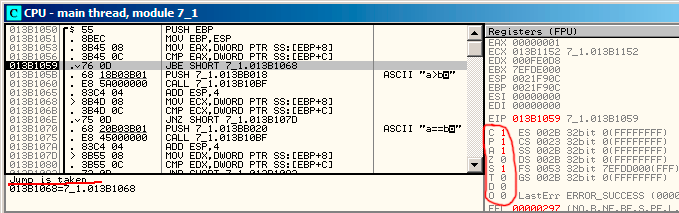
\includegraphics[scale=\FigScale]{patterns/07_jcc/olly_unsigned1.png}
\caption{\olly: \TT{f\_unsigned()}: \RU{первый условный переход}\EN{first conditional jump}}
\label{fig:jcc_olly_unsigned_1}
\end{figure}

\begin{figure}[H]
\centering
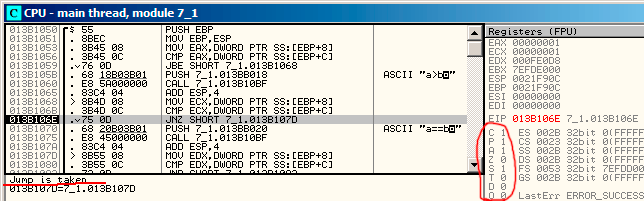
\includegraphics[scale=\FigScale]{patterns/07_jcc/olly_unsigned2.png}
\caption{\olly: \TT{f\_unsigned()}: \RU{второй условный переход}\EN{second conditional jump}}
\label{fig:jcc_olly_unsigned_2}
\end{figure}

\begin{figure}[H]
\centering
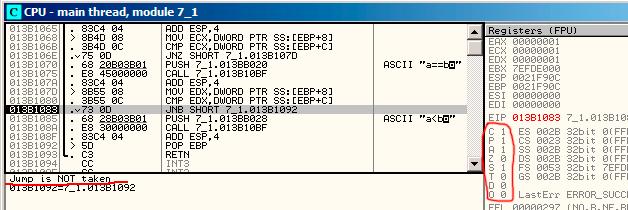
\includegraphics[scale=\FigScale]{patterns/07_jcc/olly_unsigned3.png}
\caption{\olly: \TT{f\_unsigned()}: \RU{третий условный переход}\EN{third conditional jump}}
\label{fig:jcc_olly_unsigned_3}
\end{figure}

\RU{Теперь можно попробовать в \olly ф-цию}\EN{Now we can try in \olly the} \TT{f\_signed()} 
\RU{работающую с знаковыми величинами}\EN{function working with signed values}.

\RU{Флаги выставляются точно так же}\EN{Flags are set in the same way}: 
C=1, P=1, A=1, Z=0, S=1, T=0, D=0, O=0.

\RU{Первый переход}\EN{The first conditional jump} \JLE \RU{сработает}\EN{will trigger}. 
\figref{fig:jcc_olly_signed_1}.
\RU{В}\EN{In} \cite{Intel} \RU{мы можем прочитать что эта инструкция срабатывает если}\EN{we may find
that this instruction is triggering if} 
ZF=1 \OrENRU SF$\neq$OF.
\RU{В нашем случае, }SF$\neq$OF\RU{, так что переход срабатывает}\EN{ in our case, so jump is triggering}.

\RU{Второй переход}\EN{The next} \JNZ \RU{сработает}\EN{conditional jump will trigger}: 
\RU{он срабатывает если}\EN{it does if} ZF=0 (zero flag): \figref{fig:jcc_olly_signed_2}.

\RU{Третий переход}\EN{The third conditional jump} \JGE 
\RU{не сработает, потому что он срабатывает только если}\EN{will not trigger because it will only if} SF=OF, 
\RU{что в нашем случае не так}\EN{and that is not true in our case}: \figref{fig:jcc_olly_signed_3}.

\begin{figure}[H]
\centering
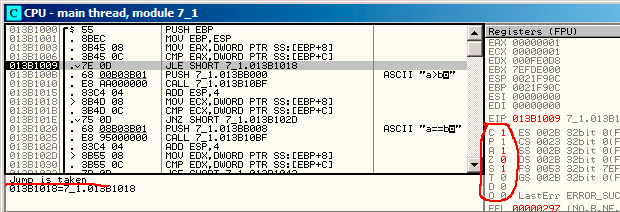
\includegraphics[scale=\FigScale]{patterns/07_jcc/olly_signed1.png}
\caption{\olly: \TT{f\_unsigned()}: \RU{первый условный переход}\EN{first conditional jump}}
\label{fig:jcc_olly_signed_1}
\end{figure}

\begin{figure}[H]
\centering
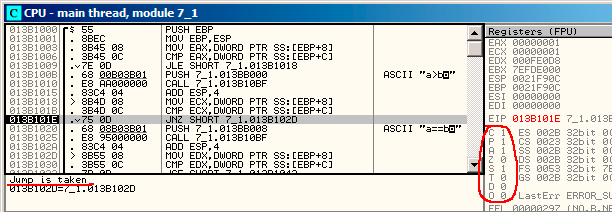
\includegraphics[scale=\FigScale]{patterns/07_jcc/olly_signed2.png}
\caption{\olly: \TT{f\_unsigned()}: \RU{второй условный переход}\EN{second conditional jump}}
\label{fig:jcc_olly_signed_2}
\end{figure}

\begin{figure}[H]
\centering
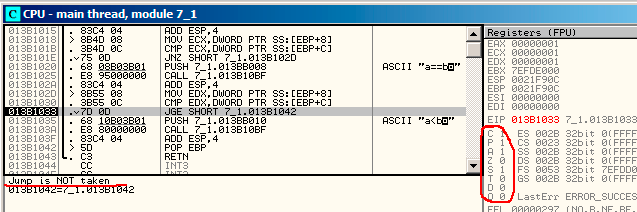
\includegraphics[scale=\FigScale]{patterns/07_jcc/olly_signed3.png}
\caption{\olly: \TT{f\_unsigned()}: \RU{третий условный переход}\EN{third conditional jump}}
\label{fig:jcc_olly_signed_3}
\end{figure}

\subsection{x86 + MSVC + Hiew}
\index{Hiew}

\RU{Можем попробовать модифицировать исполняемый файл так}\EN{We can try patch executable file in that way}, 
\RU{чтобы ф-ция}\EN{that} \TT{f\_unsigned()} \RU{всегда показывала}\EN{function will always print} ``a==b'', 
\RU{при любых входящих значениях}\EN{for any input values}.

\RU{Вот как она выглядит в}\EN{Here is how it looks in} Hiew: \figref{fig:jcc_hiew_1}.

\RU{Собственно, задаче три}\EN{Essentially, we've got three tasks}:
\begin{itemize}
\item \RU{заставить первый переход срабатывать всегда}\EN{force first jump to be always triggered};
\item \RU{заставить второй переход не срабатывать никогда}\EN{force second jump to be never triggered};
\item \RU{заставить третий переход срабатывать всегда}\EN{force third jump to be always triggered}.
\end{itemize}

\RU{Так мы направим путь исполнения кода (code flow) во второй}\EN{Thus we can point code flow
into the second} \printf,
\RU{и он всегда будет срабатывать и выводить на консоль}\EN{and it always print} ``a==b''.

\RU{Для этого нужно пропатчить три инструкции (или байта)}\EN{Three instructions (or bytes) should be patched}:

\begin{itemize}
\item \RU{Первый переход теперь будет}\EN{The first jump will now be} \JMP, \RU{но смещение перехода 
(\gls{jump offset}) останется прежним}\EN{but \gls{jump offset} will be same}.

\item \RU{Второй переход может быть и будет срабатывать иногда, но в любом случае он будет совершать переход
только на следующую инструкцию, потому что мы выставляем смещение перехода (\gls{jump offset}) в 0}
\EN{The second jump may be triggered sometimes, but in any case it will jump to the next
instruction, because, we set \gls{jump offset} to 0}.
\RU{В этих инструкциях, смещение перехода просто прибавляется к адресу следующей инструкции}
\EN{\Gls{jump offset} is just to be added to the address of the next instruction in these instructions}.
\RU{И когда смещение 0, то тогда и переход будет на следующую инструкцию}\EN{So if offset is 0,
jump will be done to the next instruction}.

\item \RU{Третий переход конвертируем в \JMP точно так же, как и первый, он будет срабатывать всегда}
\EN{The third jump we convert into \JMP just as the first one, so it will be triggered always}.
\end{itemize}

\RU{Что и делаем}\EN{That's what we do}: \figref{fig:jcc_hiew_2}.

\RU{Если забыть про какой-то из переходов, то тогда будет срабатывать несколько вызовов \printf, 
а нам ведь нужно чтобы исполнялся только один}\EN{If we could forget about any of these jumps, then several
\printf calls may execute, but this behaviour is not we're need}.

\begin{figure}[H]
\centering
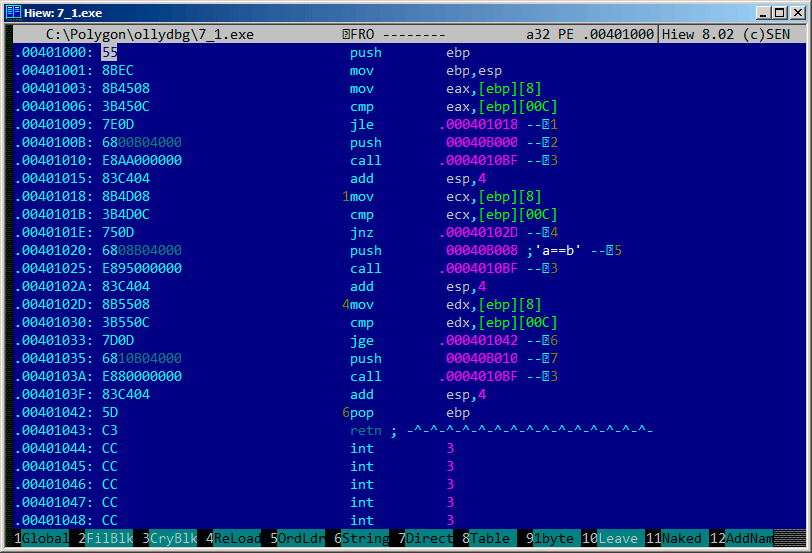
\includegraphics[scale=\FigScale]{patterns/07_jcc/hiew_unsigned1.png}
\caption{Hiew: \RU{функция }\TT{f\_unsigned()}\EN{ function}}
\label{fig:jcc_hiew_1}
\end{figure}

\begin{figure}[H]
\centering
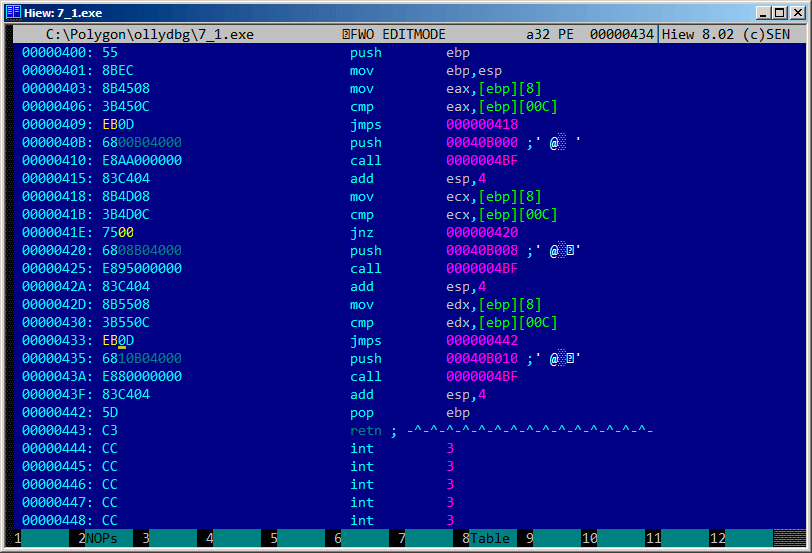
\includegraphics[scale=\FigScale]{patterns/07_jcc/hiew_unsigned2.png}
\caption{Hiew: \RU{модифицируем функцию}\EN{let's modify} \TT{f\_unsigned()}\EN{ function}}
\label{fig:jcc_hiew_2}
\end{figure}

\subsection{\NonOptimizing GCC}

\index{puts() \RU{вместо}\EN{instead of} printf()}
\NonOptimizing GCC 4.4.1 \RU{производит почти такой же код, за исключением}
\EN{produce almost the same code, but with} \puts~(\ref{puts}) \RU{вместо}\EN{instead of} \printf.

\subsection{\Optimizing GCC}

\RU{Наблюдательный читатель может спросить, зачем исполнять \CMP так много раз,
если флаги всегда одни и те же}\EN{Observant reader may ask, why to execute \CMP several times, 
if flags are same after each execution}?
\RU{По видимому, оптимизирующий MSVC не может этого делать, но GCC 4.8.1 делает больше оптимизаций}\EN{Perhaps, 
optimizing MSVC can't do this, but optimizing GCC 4.8.1 can do deep optimization}:

\lstinputlisting[caption=GCC 4.8.1 f\_signed()]{patterns/07_jcc/GCC_O3_signed.asm}

% should be here instead of 'switch' section?
\RU{Мы здесь также видим}\EN{We also see} \TT{JMP puts} \RU{вместо}\EN{here instead of} \TT{CALL puts / RETN}.
\RU{Этот прием будет описан немного позже}\EN{This kind of trick will be described later}: \ref{JMP_instead_of_RET}.

\RU{Нужно сказать что x86-код такого типа редок}\EN{Needless to say, that this type of x86 code 
is somewhat rare}.
MSVC 2012, \RU{как видно, не может генерировать подобное}\EN{as it seems, can't generate such code}.
\RU{С другой стороны, программисты на ассемблере прекрасно осведомлены о том, что инструкции}\EN{On the other hand, 
assembly language programmers are fully aware of the fact that} \TT{Jcc} \RU{можно располагать последовательно}
\EN{instructions can be stacked}.
\RU{Так что если вы видите это где-то, имеется немалая вероятность, что этот фрагмент кода был написан вручную}
\EN{So if you see it somewhere, it may be a good probability that the code is hand-written}.

\RU{Ф-ция }\TT{f\_unsigned()} \RU{получилась не настолько эстетически короткой}\EN{function is not that 
\ae{}sthetically short}:

\lstinputlisting[caption=GCC 4.8.1 f\_unsigned()]{patterns/07_jcc/GCC_O3_unsigned_\LANG.asm}

\RU{Так что, алгоритмы оптимизации}\EN{So, optimization algorithms of} GCC 4.8.1 
\RU{наверное, еще пока не идеальны}\EN{are probably not always perfect yet}.

